\documentclass[conference]{IEEEtran}
\IEEEoverridecommandlockouts

\usepackage{cite}
\usepackage[T1]{fontenc}
\usepackage{newtxtext,newtxmath}
\usepackage{amsmath}
\usepackage{graphicx}
\usepackage{booktabs}
\usepackage{xcolor}
\usepackage{url}
\usepackage{tikz}
\usetikzlibrary{arrows.meta,decorations.pathreplacing,positioning,calc}

\definecolor{msblue}{HTML}{2A78D6}
\definecolor{msorange}{HTML}{EB6834}
\newcommand{\todo}[1]{\textcolor{red}{[TODO: #1]}}

% Firmware footprint (idf.py size-components, ESP-IDF v6.1, -O2)
% generated by firmware/tools/footprint_tex.py -- do not edit
\newcommand{\FPIdsNodeCode}{2\,688}
\newcommand{\FPIdsNodeRo}{0}
\newcommand{\FPIdsNodeRam}{2\,762}
\newcommand{\FPIdsSinkCode}{5\,553}
\newcommand{\FPIdsSinkRo}{0}
\newcommand{\FPIdsSinkRam}{19\,106}
\newcommand{\FPMeshNodeCode}{4\,934}
\newcommand{\FPMeshNodeRo}{114}
\newcommand{\FPMeshNodeRam}{1\,973}
\newcommand{\FPImgCode}{538\,996}
\newcommand{\FPImgRo}{103\,360}
\newcommand{\FPImgRam}{119\,186}
\newcommand{\FPIdsNodeFlash}{2.6}


\begin{document}

\title{MeshSentry: Lightweight Collaborative Intrusion Detection for ESP-NOW Mesh Networks on the ESP32-S3}

\author{\IEEEauthorblockN{Nabil Litayem}
\IEEEauthorblockA{\todo{Department}, \todo{University}\\
\todo{City, Country}\\
nabil.litayem@gmail.com}}

\maketitle

\begin{abstract}
ESP-NOW lets low-cost ESP32 devices build connectionless multi-hop sensor
networks, but these networks have no intrusion detection: once a node is
compromised or a radio replays captured frames, the mesh silently loses data.
We present MeshSentry, an intrusion detection system (IDS) that runs on the
ESP32-S3 itself. Because every MeshSentry frame is an authenticated broadcast,
each node passively monitors its neighbours. It applies a binomial hypothesis
test to forwarding behaviour, an exponentially weighted baseline to frame rates,
a sliding anti-replay window, and a check of hop-1 route claims against a
sink-signed neighbour list. Nodes condense this evidence into 10-byte records.
The sink fuses them by trust-weighted voting with an accuser quorum and
detects Sybil identities by clustering their received-signal-strength (RSSI)
signatures across monitors. In a 25-node simulation with five attacks (selective forwarding,
sinkhole, flooding, replay, Sybil), MeshSentry detects 95--100\% of attacks
with a false-positive rate (FPR) of 0.4--3.7\%, compared with 3.7--16\% for the
same detectors without fusion and 16--25\% for a classical watchdog. Median
detection latency is 16--26\,s. Isolating detected nodes restores the packet
delivery ratio from 67\% to 90\% under a sinkhole attack, and IDS reports
occupy 0.8\% of channel airtime. The complete firmware builds with ESP-IDF
v6.1, and the IDS adds only \FPIdsNodeFlash\,kB of flash and 2.7\,kB of RAM to a sensor node.
\end{abstract}

\begin{IEEEkeywords}
Intrusion detection, ESP-NOW, ESP32-S3, wireless mesh networks, selective forwarding, Sybil attack, trust management, IoT security.
\end{IEEEkeywords}

% =====================================================================
\section{Introduction}
Espressif's ESP-NOW protocol~\cite{espnow} exchanges short vendor-specific
action frames between ESP32 devices without an access point or an association
handshake. Its low latency, its range, and the low price of chips such as the
ESP32-S3~\cite{esp32s3ds} have made it a popular basis for home-automation,
agricultural and industrial sensor meshes. These meshes are typically built
from ad-hoc relaying code. The link-layer encryption that ESP-NOW optionally
provides protects confidentiality between paired peers, but it does nothing
against an \emph{insider}: a node whose key has been extracted can drop the
traffic it should relay, advertise forged routes, inject traffic, or claim
several identities. Outsiders can still replay captured frames.

Intrusion detection for wireless sensor networks has a long history,
including watchdogs~\cite{marti2000watchdog}, reputation
systems~\cite{buchegger2002confidant,ganeriwal2008rfsn}, 6LoWPAN-oriented IDSs such as
SVELTE~\cite{raza2013svelte}, and the surveys
in~\cite{butun2014survey,zarpelao2017survey}. Most of this work assumes
TinyOS-class motes or IP-based stacks with routers that can host detection
logic. ESP-NOW meshes differ in three ways that we exploit:
(i)~frames can be broadcast so every neighbour overhears every hop;
(ii)~the ESP32-S3 has hardware SHA and big-number accelerators, so every frame can be
authenticated and control messages can carry public-key signatures; and
(iii)~it has enough RAM to keep per-neighbour statistics for dozens of neighbours.

This paper makes the following contributions:
\begin{itemize}
\item \textbf{Design.} MeshSentry, a two-tier IDS for ESP-NOW meshes. Every
node runs lightweight statistical detectors on overheard traffic, and a sink
fuses compact evidence with trust-weighted, quorum-based voting and RSSI-signature
Sybil detection (Sec.~\ref{sec:design}).
\item \textbf{Principled local tests.} We replace the fixed forwarding-ratio
threshold of the classical watchdog with a one-sided binomial test that is
normalised by the measured link quality. At the same detection rate, this cuts
the false-positive rate from 20\% to 0.2\% (Sec.~\ref{sec:eval}).
\item \textbf{Implementation.} An open ESP-IDF v6.1 firmware for the ESP32-S3
with PSA-Crypto frame authentication, ECDSA-signed control floods,
and a testbed attack-emulation module (Sec.~\ref{sec:impl}).
\item \textbf{Evaluation.} A simulation study of five attacks plus colluding
bad-mouthing monitors, including the honest finding that reputation
weighting does not help against colluders who build trust before they strike;
the accuser quorum does (Sec.~\ref{sec:eval}).
\end{itemize}

% =====================================================================
\section{Related Work}
\textbf{Watchdogs and reputation.} Marti et al.~\cite{marti2000watchdog}
proposed the watchdog/pathrater pair, in which a sender overhears its next hop and
flags it when the fraction of forwarded packets falls below a fixed threshold.
CONFIDANT~\cite{buchegger2002confidant} and RFSN~\cite{ganeriwal2008rfsn}
propagate Bayesian reputation, the latter using the Beta reputation
system~\cite{josang2002beta}, which we also adopt for monitor trust. Fixed
thresholds confuse link losses and collisions with misbehaviour. As our results show, this
gives a watchdog false-positive rates near 20\% in realistic channels.

\textbf{IoT intrusion detection.} SVELTE~\cite{raza2013svelte} places
detection in the 6LoWPAN border router and targets RPL attacks (sinkhole,
selective forwarding). Kalis~\cite{midi2017kalis} adapts its detection modules
to the network context it discovers. Surveys~\cite{butun2014survey,zarpelao2017survey}
classify placement (centralised, distributed, hybrid) and methods
(signature, anomaly, specification). MeshSentry is a hybrid,
specification- and anomaly-based design that does not depend on IP routing.

\textbf{Sybil and routing attacks.} Karlof and Wagner~\cite{karlof2003secure}
catalogue routing attacks on sensor networks, and Newsome et al.~\cite{newsome2004sybil}
analyse Sybil defences. Demirbas and Song~\cite{demirbas2006sybil} showed that
ratios of RSSI values measured by several receivers identify Sybil identities that share one radio.
We use a related RSSI-signature distance but compute it at the sink
from evidence that monitors report anyway, so it adds no traffic. Signed
control floods follow the authenticated-broadcast idea of
SPINS~\cite{perrig2002spins}, with ECDSA~\cite{fips186-5} instead of $\mu$TESLA,
which the S3 can afford.

To the best of our knowledge, no prior work provides an IDS for ESP-NOW
meshes, or an evaluated IDS implementation for the ESP32 family.
\todo{verify novelty claim against 2024--2026 literature}

% =====================================================================
\section{System and Threat Model}
\label{sec:model}
\textbf{Network.} $N$ static ESP32-S3 nodes report sensor data to a
trusted sink over multiple hops. All frames are ESP-NOW broadcasts carrying the
intended next hop, so any neighbour can overhear them. Routing is an ETX
gradient~\cite{decouto2003etx}. Members share a network key $K$, which they
use to authenticate frames with a truncated HMAC. The sink holds an
ECDSA-P256 key pair whose public key is provisioned on all nodes.

\textbf{Adversary.} We consider (a)~\emph{insiders}: compromised members
that know $K$ and run arbitrary firmware; and (b)~\emph{outsiders} without
$K$ that can record and retransmit frames. The attacks are
\emph{selective forwarding} (dropping relayed frames with probability $p$),
\emph{sinkhole} (claiming a one-hop route to the sink and then dropping
everything), \emph{flooding} (authenticated junk at hundreds of frames/s),
\emph{replay} (verbatim retransmission of captured frames), and
\emph{Sybil} (beacons under several fabricated identities). We also consider
\emph{colluding bad-mouthers}: compromised monitors that report false evidence
against one honest node. Physical-layer jamming and compromise of the sink are out of scope.

% =====================================================================
\section{MeshSentry Design}
\label{sec:design}
\begin{figure*}[t]
\centering
% System architecture of MeshSentry (figure*).
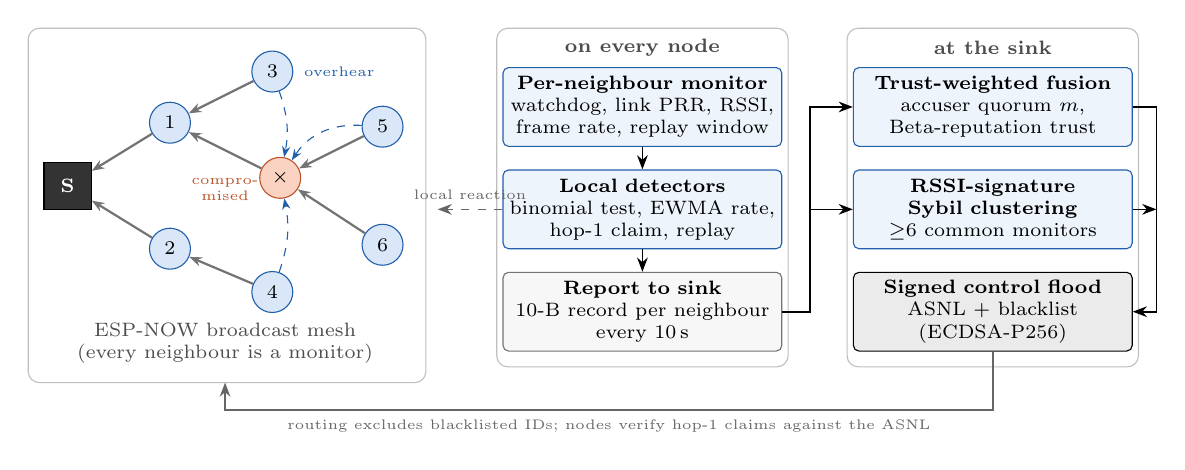
\begin{tikzpicture}[
  font=\footnotesize,
  node/.style={circle, draw=msblue!80!black, fill=msblue!18, minimum size=5.2mm, inner sep=0pt, font=\scriptsize},
  sink/.style={rectangle, draw=black, fill=black!80, text=white, minimum size=6mm, inner sep=0pt, font=\scriptsize\bfseries},
  bad/.style={circle, draw=msorange!80!black, fill=msorange!30, minimum size=5.2mm, inner sep=0pt, font=\scriptsize},
  blk/.style={rectangle, rounded corners=2pt, draw=black!55, fill=black!3, align=center,
              minimum height=10mm, text width=34mm, inner sep=2pt, font=\scriptsize},
  hl/.style={blk, draw=msblue!80!black, fill=msblue!8},
  route/.style={-{Stealth[length=1.6mm]}, thick, black!55},
  over/.style={dashed, msblue!80!black, -{Stealth[length=1.4mm]}},
  flow/.style={-{Stealth[length=1.8mm]}, semithick},
]
% ---------------- left: mesh
\node[sink] (S) at (0,0) {S};
\node[node] (a) at (1.3,0.8) {1};
\node[node] (b) at (1.3,-0.8) {2};
\node[bad]  (x) at (2.7,0.1) {$\times$};
\node[node] (c) at (2.6,1.45) {3};
\node[node] (d) at (2.6,-1.35) {4};
\node[node] (e) at (4.0,0.75) {5};
\node[node] (f) at (4.0,-0.75) {6};
\draw[route] (a) -- (S);
\draw[route] (b) -- (S);
\draw[route] (x) -- (a);
\draw[route] (c) -- (a);
\draw[route] (d) -- (b);
\draw[route] (e) -- (x);
\draw[route] (f) -- (x);
\draw[over] (c) to[bend left=15] (x);
\draw[over] (d) to[bend right=15] (x);
\draw[over] (e) to[bend right=30] (x);
\node[font=\tiny, msblue!80!black] at (3.45,1.45) {overhear};
\node[font=\tiny, msorange!80!black, align=center] at (2.0,-0.05) {compro-\\mised};
\node[font=\scriptsize, align=center, text=black!70] at (2.0,-2.0)
  {ESP-NOW broadcast mesh\\(every neighbour is a monitor)};
\draw[black!25, rounded corners] (-0.5,-2.5) rectangle (4.55,2.0);

% ---------------- middle: every node
\node[font=\scriptsize\bfseries, text=black!70] at (7.3, 1.75) {on every node};
\node[hl]  (mon) at (7.3, 1.0)  {\textbf{Per-neighbour monitor}\\watchdog, link PRR, RSSI,\\frame rate, replay window};
\node[hl]  (det) at (7.3,-0.3) {\textbf{Local detectors}\\binomial test, EWMA rate,\\hop-1 claim, replay};
\node[blk] (rep) at (7.3,-1.6) {\textbf{Report to sink}\\10-B record per neighbour\\every 10\,s};
\draw[flow] (mon) -- (det);
\draw[flow] (det) -- (rep);
\draw[black!25, rounded corners] (5.45,-2.3) rectangle (9.15,2.0);
\draw[flow, dashed, black!60] (det.west) -- (4.7,-0.3) node[midway, above, font=\tiny] {local reaction};

% ---------------- right: sink
\node[font=\scriptsize\bfseries, text=black!70] at (11.75, 1.75) {at the sink};
\node[hl]  (fus) at (11.75, 1.0)  {\textbf{Trust-weighted fusion}\\accuser quorum $m$,\\Beta-reputation trust};
\node[hl]  (syb) at (11.75,-0.3) {\textbf{RSSI-signature}\\\textbf{Sybil clustering}\\$\geq$6 common monitors};
\node[blk, draw=black, fill=black!8] (ctl) at (11.75,-1.6) {\textbf{Signed control flood}\\ASNL + blacklist\\(ECDSA-P256)};
\draw[black!25, rounded corners] (9.9,-2.3) rectangle (13.6,2.0);
\draw[flow] (rep.east) -- ++(0.35,0) |- (fus.west);
\draw[flow] (rep.east) -- ++(0.35,0) |- (syb.west);
\draw[flow] (fus.east) -- ++(0.3,0) |- (ctl.east);
\draw[flow] (syb.east) -- ++(0.3,0);
\draw[flow, black!60] (ctl.south) -- (11.75,-2.85) -- node[below, font=\tiny]
  {routing excludes blacklisted IDs; nodes verify hop-1 claims against the ASNL} (2.0,-2.85) -- (2.0,-2.5);
\end{tikzpicture}

\caption{MeshSentry architecture. Every node monitors the neighbours it
overhears and runs local detectors. Every 10\,s it sends one compact record per
neighbour to the sink, which fuses the records with trust-weighted, quorum-based voting, clusters
RSSI signatures to expose Sybil identities, and floods an ECDSA-signed control
message carrying the authenticated sink-neighbour list (ASNL) and the blacklist.}
\label{fig:arch}
\end{figure*}

Fig.~\ref{fig:arch} gives an overview of the design. Time is divided into
windows of $W=10$\,s aligned to the sink clock. Each signed control frame
carries the sink's time, which nodes use to align their windows.

\subsection{Authenticated Broadcast Mesh}
Fig.~\ref{fig:frame} shows the frame format. A 16-byte header carries the
transmitter \texttt{tx}, a per-transmitter sequence number \texttt{txseq}, the
originator and its end-to-end sequence number, the next hop, the hop count, and
the payload length. A 64-bit truncated HMAC-SHA256 tag covers the header and
payload. Receivers check \texttt{txseq} against a 64-entry sliding window,
as in IPsec anti-replay~\cite{rfc4303}. The upper bits of \texttt{txseq} hold a
boot epoch stored in flash, so a rebooted node is not mistaken for a replayer.
Beacons advertise the path ETX. A node that loses its route keeps
beaconing with infinite cost (\emph{route poisoning}), so its neighbours
do not expect it to forward.
Every 10\,s the sink floods a control frame signed with ECDSA-P256. It
contains the \emph{authenticated sink-neighbour list} (ASNL), i.e.\ the nodes
the sink actually hears, and the current blacklist.

\begin{figure}[t]
\centering
% Frame and report-record formats (single column).
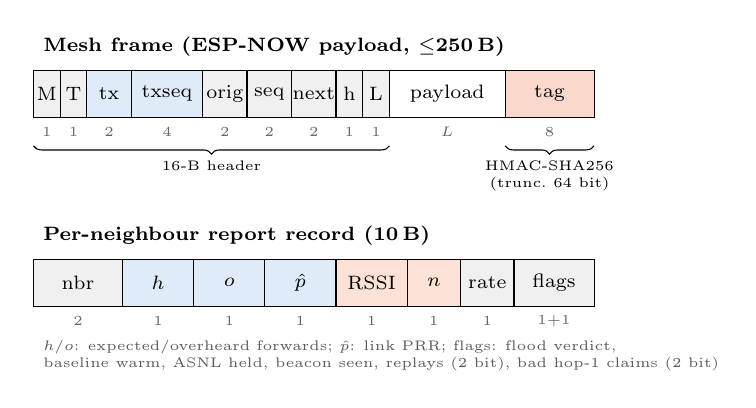
\begin{tikzpicture}[font=\scriptsize, x=0.565mm, y=1mm]
  \newcommand{\fld}[5]{% x, width, label, bytes, fill
    \draw[fill=#5] (#1,0) rectangle ++(#2,6);
    \node at (#1+#2/2,3) {#3};
    \node[font=\tiny, black!60] at (#1+#2/2,-1.8) {#4};}
  \node[anchor=west, font=\scriptsize\bfseries] at (0,9) {Mesh frame (ESP-NOW payload, $\leq$250\,B)};
  \fld{0}{6}{M}{1}{black!6}
  \fld{6}{6}{T}{1}{black!6}
  \fld{12}{10}{tx}{2}{msblue!15}
  \fld{22}{16}{txseq}{4}{msblue!15}
  \fld{38}{10}{orig}{2}{black!6}
  \fld{48}{10}{seq}{2}{black!6}
  \fld{58}{10}{next}{2}{black!6}
  \fld{68}{6}{h}{1}{black!6}
  \fld{74}{6}{L}{1}{black!6}
  \fld{80}{26}{payload}{$L$}{white}
  \fld{106}{20}{tag}{8}{msorange!25}
  \draw[decorate, decoration={brace, amplitude=3pt, mirror}] (0,-3.6) -- (80,-3.6)
     node[midway, below=2pt, font=\tiny] {16-B header};
  \draw[decorate, decoration={brace, amplitude=3pt, mirror}] (106,-3.6) -- (126,-3.6)
     node[midway, below=2pt, font=\tiny, align=center] {HMAC-SHA256\\(trunc.\ 64 bit)};

  \begin{scope}[yshift=-24mm]
  \node[anchor=west, font=\scriptsize\bfseries] at (0,9) {Per-neighbour report record (10\,B)};
  \fld{0}{20}{nbr}{2}{black!6}
  \fld{20}{16}{$h$}{1}{msblue!15}
  \fld{36}{16}{$o$}{1}{msblue!15}
  \fld{52}{16}{$\hat p$}{1}{msblue!15}
  \fld{68}{16}{RSSI}{1}{msorange!20}
  \fld{84}{12}{$n$}{1}{msorange!20}
  \fld{96}{12}{rate}{1}{black!6}
  \fld{108}{18}{flags}{1+1}{black!6}
  \node[anchor=west, font=\tiny, black!65, align=left] at (0,-6.2)
   {$h$/$o$: expected/overheard forwards; $\hat p$: link PRR; flags: flood verdict,\\
    baseline warm, ASNL held, beacon seen, replays (2 bit), bad hop-1 claims (2 bit)};
  \end{scope}
\end{tikzpicture}

\caption{MeshSentry frame and per-neighbour report record.}
\label{fig:frame}
\end{figure}

\subsection{Per-Neighbour Monitoring and Local Detectors}
For each neighbour $j$, a monitor $i$ keeps an exponentially weighted
estimate of the beacon reception ratio $\hat p_{j}$ (the PRR of link
$j\!\to\!i$). It also keeps the mean RSSI and frame rate in the current window
and watchdog counters.

\textbf{Selective forwarding.} Whenever $i$ sends or overhears a data or
report frame whose next hop is $j$ (and $j$ is not the sink), it expects to
overhear $j$ forward that frame within 400\,ms. Third-party monitors take part
only if $\hat p_j \ge 0.7$. Over a sliding window of three windows, let
$h$ be the number of forwards expected and $o$ the number actually overheard.
If $j$ is honest, each expected forward is overheard with probability at
least $q\,\hat p_j$, where $q=0.9$ conservatively accounts for losses on the
upstream link. Monitor $i$ raises an alert if
\begin{equation}
F_{\mathrm{Bin}}\!\left(o;\,h,\,q\hat p_j\right)=\sum_{k=0}^{o}\binom{h}{k}(q\hat p_j)^k(1-q\hat p_j)^{h-k} < \alpha ,
\label{eq:binom}
\end{equation}
with $h\ge 6$ and $\alpha=10^{-3}$. Unlike a fixed ratio threshold,
(\ref{eq:binom}) adapts to link quality and to the amount of evidence.

\textbf{Flooding.} The per-neighbour rate $r_t$ (frames/s) is compared with
an EWMA baseline $\mu$ and a mean absolute deviation $\sigma$:
\begin{equation}
r_t > \max\!\left(r_{\min},\ \mu_{t-1} + k\max(\sigma_{t-1},0.5)\right),
\end{equation}
with $k=4$ and $r_{\min}=5$ frames/s. While an alert is active, the baseline
is not updated, so an attacker cannot drag the baseline upward.

\textbf{Forged routes.} A beacon that claims hop count 1 from a node absent
from the last two signed ASNLs counts as a bad claim. An alert is raised after
two bad claims in one window.

\textbf{Replay.} Frames that pass authentication but fail the freshness
window are dropped and counted. Two or more in one window raise a replay
alert. The alert names the identity being replayed but never blames it.

\textbf{Local reaction.} A node immediately stops routing through a neighbour
for which it raised a forwarding alert, without waiting for the sink.

\subsection{Evidence Reporting}
At the end of each window, a node sends one report to the sink containing up
to 16 ten-byte records (Fig.~\ref{fig:frame}), with records that carry alerts
first. The sink re-applies the forwarding test to the raw $(h,o,\hat p)$
values, so thresholds can be retuned centrally without reflashing the nodes.

\subsection{Sink Fusion}
For a suspect $j$ and alert class $c$, let $E$ be the monitors whose records
are \emph{eligible} for $c$ (e.g.\ $h\ge 6$ for forwarding), and let $A
\subseteq E$ be those that accuse $j$. With monitor trust $\tau_i$, the sink
declares $j$ malicious if
\begin{equation}
\frac{\sum_{i\in A}\tau_i}{\sum_{i\in E}\tau_i}\ \ge\ \theta_v,\qquad
\sum_{i\in A}\tau_i \ge M,\qquad |A|\ \ge\ m ,
\label{eq:vote}
\end{equation}
with $\theta_v=0.5$, $M=0.9$, and an \emph{accuser quorum} $m=3$. For replay,
the evidence is cryptographic, so the fraction condition is dropped. Trust is
the expected value of a Beta reputation~\cite{josang2002beta},
$\tau_i=(a_i+1)/(a_i+b_i+2)$. A monitor's $a_i$ ($b_i$) is incremented when it
agrees (disagrees) with a clear-cut outcome, defined as a score $\ge 0.75$ or
$\le 0.25$.

\textbf{Sybil detection.} Identities that share one radio produce
nearly identical mean RSSI at every monitor. For identities $a,b$ heard by a
common monitor set $\mathcal M_{ab}$ with $|\mathcal M_{ab}|\ge 6$, the sink computes
\begin{equation}
d_{ab}=\sqrt{\frac{1}{|\mathcal M_{ab}|}\sum_{i\in\mathcal M_{ab}}\left(\bar r_{ia}-\bar r_{ib}\right)^2}
\end{equation}
and flags both identities if $d_{ab}<\delta=1.5$\,dB in two of the last three
windows. Monitors with $\tau_i<0.4$ are excluded.

\textbf{Response.} Nodes that are declared malicious are added to the
blacklist in the next signed control flood. Nodes then exclude them from
parent selection.

% =====================================================================
\section{Implementation on the ESP32-S3}
\label{sec:impl}
\begin{figure}[t]
\centering
% Firmware architecture on the ESP32-S3 (single column).
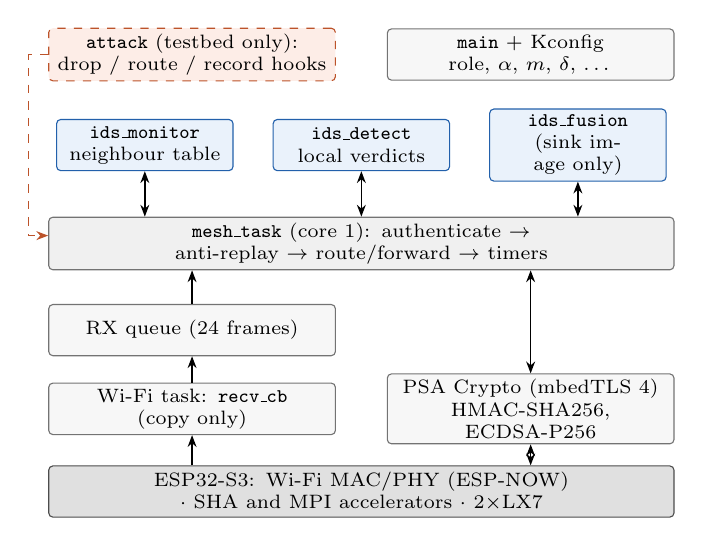
\begin{tikzpicture}[
  font=\scriptsize,
  b/.style={rectangle, rounded corners=1.5pt, draw=black!55, fill=black!3, align=center, minimum height=6.5mm, inner sep=2pt},
  ids/.style={b, draw=msblue!80!black, fill=msblue!10, text width=21mm},
  hw/.style={b, draw=black!70, fill=black!12},
  att/.style={b, draw=msorange!80!black, fill=msorange!12, dashed},
  ar/.style={-{Stealth[length=1.5mm]}, semithick},
  dar/.style={{Stealth[length=1.5mm]}-{Stealth[length=1.5mm]}, semithick},
]
\node[hw, text width=78mm] (hw) at (0,0) {ESP32-S3: Wi-Fi MAC/PHY (ESP-NOW) $\cdot$ SHA and MPI accelerators $\cdot$ 2$\times$LX7};
\node[b, text width=35mm] (wifi) at (-2.15,1.05) {Wi-Fi task: \texttt{recv\_cb} (copy only)};
\node[b, text width=35mm] (psa) at (2.15,1.05) {PSA Crypto (mbedTLS 4)\\HMAC-SHA256, ECDSA-P256};
\node[b, text width=35mm] (q) at (-2.15,2.05) {RX queue (24 frames)};
\node[b, text width=78mm, fill=black!6] (task) at (0,3.15)
   {\textbf{\texttt{mesh\_task}} (core 1): authenticate $\to$ anti-replay $\to$ route/forward $\to$ timers};
\node[ids] (mon) at (-2.75,4.4) {\texttt{ids\_monitor}\\neighbour table};
\node[ids] (det) at (0,4.4) {\texttt{ids\_detect}\\local verdicts};
\node[ids] (fus) at (2.75,4.4) {\texttt{ids\_fusion}\\(sink image only)};
\node[att, text width=35mm] (att) at (-2.15,5.55) {\texttt{attack} (testbed only):\\drop / route / record hooks};
\node[b, text width=35mm] (cfg) at (2.15,5.55) {\texttt{main} + Kconfig\\role, $\alpha$, $m$, $\delta$, \dots};
\draw[ar] (hw.north -| wifi) -- (wifi);
\draw[ar] (wifi) -- (q);
\draw[ar] (q) -- (q |- task.south);
\draw[dar] (psa) -- (psa |- task.south);
\draw[dar] (psa.south) -- (hw.north -| psa);
\draw[dar] (mon.south) -- (mon.south |- task.north);
\draw[dar] (det.south) -- (det.south |- task.north);
\draw[dar] (fus.south) -- (fus.south |- task.north);
\draw[ar, dashed, msorange!80!black] (att.west) -- ++(-0.25,0) |- ([yshift=1mm]task.west);
\end{tikzpicture}

\caption{Firmware architecture. The Wi-Fi task only copies received frames;
all protocol and IDS state is owned by one task, so no locks are needed on
the hot path.}
\label{fig:fw}
\end{figure}

The firmware (Fig.~\ref{fig:fw}) targets ESP-IDF v6.1 and consists of five
components: \texttt{proto} (wire format), \texttt{mesh} (ESP-NOW transport,
routing, control plane), \texttt{ids} (monitor, detectors, fusion),
\texttt{attack} (testbed emulation), and \texttt{main}. Authentication uses
the PSA Crypto API of mbedTLS~4: \texttt{psa\_mac\_verify} with a truncated
HMAC-SHA256 algorithm, which runs on the S3's SHA accelerator, and
\texttt{psa\_sign/verify\_message} with ECDSA-P256 for control frames. The node
role (sink, node, or attacker), the attack type, and every threshold
($\alpha$, $m$, $\delta$, \dots) are Kconfig options, and one script builds
all seven role images. Fusion code and tables are compiled only into the sink image, so the IDS adds \FPIdsNodeFlash\,kB of flash and 2.7\,kB of RAM to a sensor node. The sink's fusion tables (reports from 32 monitors over two windows, trust, vote and Sybil-pair state) take 19\,kB, which is under 6\% of the S3's 512\,kB SRAM.

Table~\ref{tab:footprint} lists the memory footprint measured with
\texttt{idf.py size-components}. Per-node IDS state is statically allocated:
24 neighbour entries, 48 pending watchdog expectations, and an anti-replay bitmap per neighbour.
The attack module reproduces the simulated attackers with behaviour hooks
(drop, route rewrite, raw-frame recording), so the same experiments can be run
on hardware.

\begin{table}[t]
\centering
\caption{Firmware footprint on the ESP32-S3 (bytes, ESP-IDF v6.1, \texttt{-O2}); whole-image RAM includes code placed in internal RAM}
\label{tab:footprint}
\begin{tabular}{lrrr}
\toprule
Component & Flash code & Flash data & Static RAM \\
\midrule
\texttt{ids} (sensor node) & \FPIdsNodeCode & \FPIdsNodeRo & \FPIdsNodeRam \\
\texttt{ids} (sink, with fusion) & \FPIdsSinkCode & \FPIdsSinkRo & \FPIdsSinkRam \\
\texttt{mesh} (sensor node) & \FPMeshNodeCode & \FPMeshNodeRo & \FPMeshNodeRam \\
\midrule
Whole image (sensor node) & \FPImgCode & \FPImgRo & \FPImgRam \\
\bottomrule
\end{tabular}
\end{table}

% =====================================================================
\section{Evaluation}
\label{sec:eval}
\subsection{Methodology}
We evaluate MeshSentry with a discrete-event simulator that models the
same protocol and runs a Python reference implementation of the detectors
that mirrors the C firmware's logic and thresholds. Table~\ref{tab:setup} lists the parameters.
The radio model uses log-distance path loss with symmetric static
shadowing~\cite{rappaport2002wireless}, per-frame fading, and a sigmoid
reception curve that reproduces the transitional
region~\cite{zuniga2004transitional}. The MAC model includes carrier sensing,
collisions with a 4\,dB capture threshold, and half-duplex radios. The attacker
(a single node) is compromised at $t=150$\,s. For selective forwarding and
sinkhole it is the relay with the largest subtree, which is the worst case.
Fig.~\ref{fig:topo} shows a sample topology.

All thresholds were calibrated on a separate set of ten seeds. Every result
uses 20 fresh seeds per scenario. We report the \emph{detection rate} (the
fraction of runs in which the attacker is declared after onset) and the
\emph{false-positive rate} (FPR, the fraction of honest nodes that are ever
declared malicious during the 400\,s run). We compare against
(i)~\emph{Local-only}: the same detectors, but any single honest monitor's
alert counts; and (ii)~the classical \emph{Watchdog}~\cite{marti2000watchdog}:
a sender flags its next hop if fewer than 50\% of the frames it handed over
are overheard being forwarded.

\begin{table}[t]
\centering
\caption{Simulation parameters}
\label{tab:setup}
\small
\begin{tabular}{@{}ll@{}}
\toprule
Topology & 25 nodes, $5{\times}5$ grid, 15\,m pitch, $\pm$3\,m jitter \\
Radio & 0\,dBm, $PL_0$=40\,dB, $n$=3.3, $\sigma_s$=4\,dB, $\sigma_f$=1.5\,dB \\
Reception & sens.\ $-88$\,dBm, CS $-92$\,dBm, 1\,Mb/s ESP-NOW \\
Traffic & beacon 2\,s, data 5\,s/node, report 10\,s/node \\
Run & 400\,s, attack at 150\,s, 20 seeds/scenario \\
Attacks & drop $p$=0.6; flood 300\,f/s; replay 4\,f/s; 4 Sybil IDs \\
IDS & $W$=10\,s, $\alpha$=$10^{-3}$, $m$=3, $\theta_v$=0.5, $\delta$=1.5\,dB \\
\bottomrule
\end{tabular}
\end{table}

\begin{figure}[t]
\centering
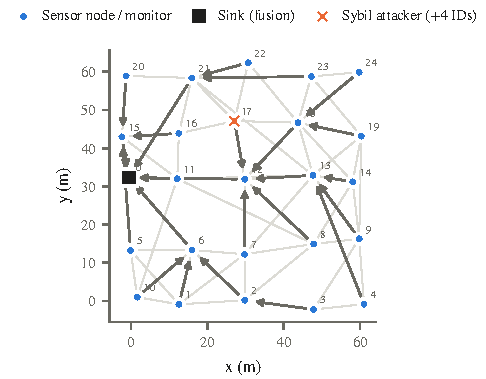
\includegraphics[width=\columnwidth]{figures/topology.pdf}
\caption{A simulated topology. Arrows show the ETX routing tree towards the sink (node 0) and grey lines show usable links. In this seed node 17 is a Sybil attacker.}
\label{fig:topo}
\end{figure}

\subsection{Detection Performance}
Fig.~\ref{fig:det} summarises the main results. MeshSentry detects the
attacker in 100\% of runs for selective forwarding, flooding, replay, and Sybil,
and in 95\% of runs for sinkhole. Its FPR stays between 0.4\% and 1.5\%, except
under flooding (3.7\%). Without flooding, honest nodes are only rarely accused.
Flooding raises the FPR because the collisions it causes make honest relays
appear to drop frames, and that effect is real rather than a modelling artefact.
Local-only detection has the same sensitivity but a 3.7--16\% FPR: across all
120 runs, single-monitor forwarding alerts accuse 194 honest (run, node) pairs,
versus 18 after fusion. Moreover, a single-monitor RSSI
comparison cannot detect Sybil identities without flagging nearly every node.
The watchdog misses flooding and replay entirely (it observes only forwarding),
and its fixed threshold yields a 16--25\% FPR.

\begin{figure}[t]
\centering
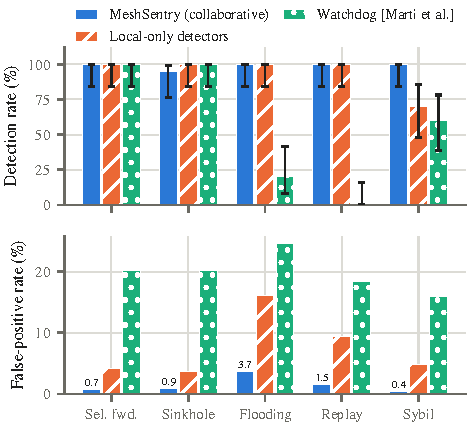
\includegraphics[width=\columnwidth]{figures/detection_fpr.pdf}
\caption{Detection rate (top, 95\% Wilson intervals) and false-positive rate
(bottom) per attack, 20 runs each.}
\label{fig:det}
\end{figure}

Fig.~\ref{fig:roc} sweeps the forwarding test's significance level
$\alpha$ (and the watchdog's threshold) for selective forwarding.
At $\alpha=10^{-3}$, MeshSentry reaches 100\% detection at 0.2\% FPR. Reaching
100\% detection with the watchdog costs 8.8\% FPR.
For forwarding alone, the binomial test is the main source of the gain: with
a very strict $\alpha$, local-only detection is equally good. The quorum
$m=3$ costs some sensitivity at very small $\alpha$ (90--95\% detection), in
exchange for resistance to bad-mouthing (Sec.~\ref{sec:badmouth}) and a
single network-wide verdict.

\begin{figure}[t]
\centering
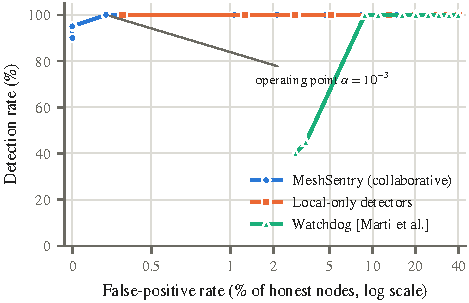
\includegraphics[width=\columnwidth]{figures/roc_selfwd.pdf}
\caption{Detection rate versus FPR for selective forwarding, obtained by sweeping
$\alpha\in[10^{-6},0.4]$ (MeshSentry, local) and the ratio threshold (watchdog).}
\label{fig:roc}
\end{figure}

Fig.~\ref{fig:drop} varies the attacker's drop probability. Grayholes that drop
40\% or more of relayed frames are detected in at least 90\% of runs. A
20\% grayhole is the hardest case: MeshSentry detects it in 65\% of runs,
compared with 85\% for local-only detection. This is the expected cost of the
quorum. Local-only detection, however, pays a 3--5\% FPR, and the watchdog
13--14\%, whereas MeshSentry stays below 0.7\%.

\begin{figure}[t]
\centering
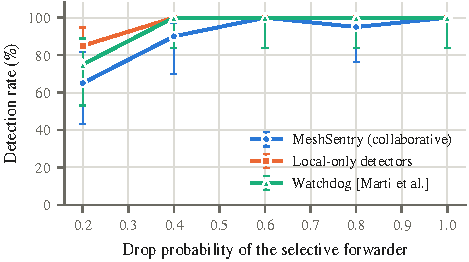
\includegraphics[width=\columnwidth]{figures/droprate.pdf}
\caption{Detection rate versus the selective forwarder's drop probability.}
\label{fig:drop}
\end{figure}

\textbf{Latency.} Detection latency (Fig.~\ref{fig:lat}) is quantised by the
10\,s window plus the 6\,s fusion delay. Flooding and replay are declared
in the first fusion round (16\,s). Forwarding attacks need evidence to
accumulate ($h\ge 6$): their median latency is 26\,s and the 90th percentile is 42\,s.

\begin{figure}[t]
\centering
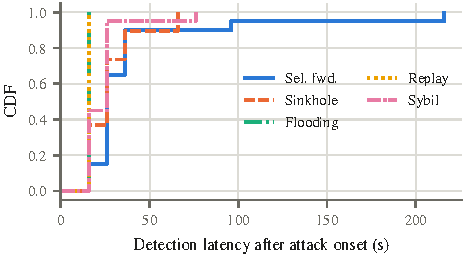
\includegraphics[width=\columnwidth]{figures/latency_cdf.pdf}
\caption{CDF of detection latency after attack onset.}
\label{fig:lat}
\end{figure}

\textbf{Sybil signatures.} Fig.~\ref{fig:sybil} shows the distribution of
$d_{ab}$. Of the pairs formed by Sybil identities and their host, 99.1\% fall
below $\delta=1.5$\,dB (99th percentile 1.46\,dB), compared with only 0.03\%
of honest pairs. The two-of-three-windows persistence rule then removes the
remaining honest coincidences.

\begin{figure}[t]
\centering
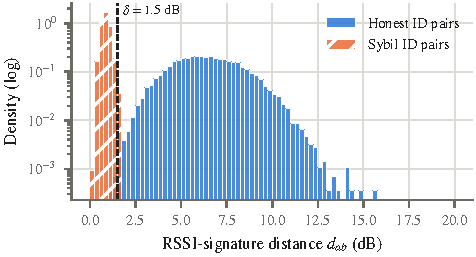
\includegraphics[width=\columnwidth]{figures/sybil_signature.pdf}
\caption{RSSI-signature distance between identity pairs observed by at least six common monitors.}
\label{fig:sybil}
\end{figure}

\subsection{Resistance to Bad-Mouthing}
\label{sec:badmouth}
In the bad-mouthing experiment, a fraction of nodes collude. Each colluder
reports fabricated evidence that one common honest victim is dropping frames,
inventing records if necessary, while a selective forwarder is also active.
Fig.~\ref{fig:bm} shows that the quorum $m=3$ is the effective safeguard. With
10\% colluders (two nodes), the FPR drops to 0.2\%, compared with 4.7\% for
$m=1$. Beyond 20\% colluders, they outnumber the honest monitors eligible to
judge the victim, and the FPR rises to 6--7\%. Trust weighting gives
\emph{no} measurable benefit (the curves coincide). The colluders behave
honestly until they strike, so they earn the same reputation as honest
monitors, and a Beta reputation only discounts them once they are outvoted.
We report this negative result because reputation is widely assumed to
counter collusion.

\begin{figure}[t]
\centering
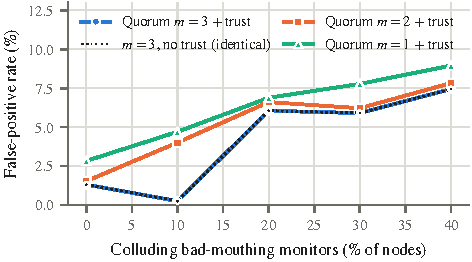
\includegraphics[width=\columnwidth]{figures/badmouth.pdf}
\caption{FPR under colluding bad-mouthing monitors for different accuser quorums $m$.}
\label{fig:bm}
\end{figure}

\subsection{Mitigation}
With blacklisting and local reaction enabled, Fig.~\ref{fig:pdr} shows the
mean packet delivery ratio (PDR) of honest originators. Under the sinkhole
attack, the PDR without isolation falls from 90.3\% to 67.0\%. With isolation
it recovers within about 30\,s to 89.8\%, the pre-attack level. A 60\%
grayhole reduces the PDR to 78.9\% without isolation and to 89.7\% with it.

\begin{figure}[t]
\centering
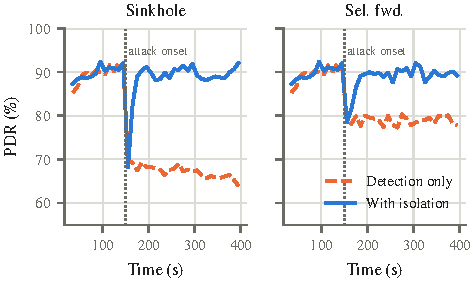
\includegraphics[width=\columnwidth]{figures/pdr_mitigation.pdf}
\caption{Packet delivery ratio over time (mean of 20 runs) with and without isolation of detected nodes.}
\label{fig:pdr}
\end{figure}

\subsection{Overhead}
Fig.~\ref{fig:ovh} breaks the channel airtime down by frame type for networks
of 16--49 nodes. IDS reports use 0.8\% of airtime at 25 nodes and 2.0\% at 49
nodes, which is comparable to the beacons. Total channel use stays below 7\%.
Reports grow faster than other traffic because they are relayed over more hops
in larger networks. Sending reports every second window, or only when the
content changes, would halve this cost.
On the nodes, the IDS adds the memory listed in Table~\ref{tab:footprint} and one
HMAC verification per received frame, which is already required for
authentication. \todo{measure per-frame CPU time and current draw on hardware}

\begin{figure}[t]
\centering
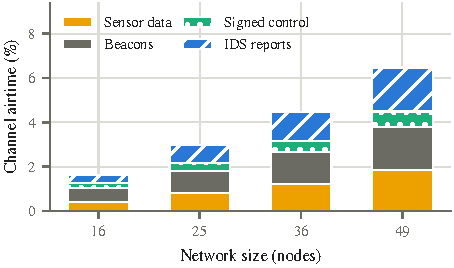
\includegraphics[width=\columnwidth]{figures/overhead.pdf}
\caption{Channel airtime by frame type versus network size (no attack).}
\label{fig:ovh}
\end{figure}

% =====================================================================
\section{Discussion and Limitations}
\textbf{Simulation versus hardware.} All quantitative results come from
simulation. The firmware is complete and compiles for every role, but has not
yet been evaluated on a physical testbed. Real ESP-NOW links may show
asymmetry, interference from Wi-Fi traffic, and RSSI quantisation that the
channel model does not capture.
\todo{add 15--20 node ESP32-S3 testbed results using the provided attack images}

\textbf{RSSI manipulation.} A Sybil attacker that randomises its transmit
power per identity can defeat absolute RSSI signatures. Using ratios of RSSI
across monitors~\cite{demirbas2006sybil}, or channel state information
(available on the ESP32-S3), is a natural extension. The Sybil detector also
assumes static nodes.

\textbf{Collusion.} The accuser quorum bounds the damage of small coalitions,
but colluders who outnumber a victim's honest neighbours can still frame it.
Cross-checking accusations against the victim's own reports (for example,
the symmetry of the RSSI the two endpoints report for their link) is future work.

\textbf{Trust anchors.} The sink and the provisioning of the network key are
trusted. In deployment, the key would live in an eFuse key block used by the
S3's HMAC peripheral rather than in flash.

% =====================================================================
\section{Conclusion}
MeshSentry shows that ESP-NOW meshes can detect insider and outsider attacks
on the nodes themselves. Authenticated broadcast turns every neighbour into
a monitor. A binomial forwarding test, a rate baseline, signed route
references, and anti-replay windows provide cheap local evidence, and a
quorum-based fusion at the sink turns that evidence into accurate, network-wide
verdicts, including Sybil detection. In simulation, MeshSentry detects
95--100\% of five attack types at 0.4--3.7\% FPR, restores delivery after
isolating attackers, and costs under 1\% of airtime at 25 nodes. The next
steps are a hardware testbed evaluation and RSSI-ratio Sybil signatures.

\section*{Artifact Availability}
The ESP-IDF firmware, simulator, experiment scripts, and figure generation
code will be released at \todo{repository URL}.

\bibliographystyle{IEEEtran}
\bibliography{refs}

\end{document}
